% LaTeX Template for short student reports.
% Citations should be in bibtex format and go in references.bib
\documentclass[a4paper, 12pt]{article}
\usepackage[top=2cm, bottom=3cm, left = 2cm, right = 2cm]{geometry} 
\geometry{a4paper} 
\usepackage[utf8]{inputenc}
\usepackage{textcomp}
\usepackage{graphicx} 
\usepackage{amsmath,amssymb}  
\usepackage{bm}  
\usepackage{memhfixc} 
\usepackage{fancyhdr}
\usepackage{float}
\usepackage{booktabs}
\usepackage{listings}
\usepackage{xcolor}
\usepackage{xepersian}
\lstset{escapeinside={<@}{@>}}
\settextfont[Scale=1.]{HM FNazli}
\setlatintextfont[Scale=.9]{Noto Sans}
\pagestyle{fancy}

\title{\lr{JOS Execution Environment}}
\author{
    علی کریمی \and
    حسین افکار \and
    محمدرضا ولی
    }
%\date{}

\begin{document}
\maketitle
در مرحله اول این تمرین ما باید هسته این سیستم‌عامل را کامپایل کرده و سپس بر روی شبیه‌ساز
\lr{QEMU}
اجرا کنیم.
برای این کار ابتدا باید دستور
\lr{make qemu}
را اجرا کنیم تا هسته کرنل ساخته شود.
این دستور ابتدا کرنل را ساخته و سپس توسط کامند مطرح شده در
\lr{Makefile}
این هسته را اجرا می‌کند.
در ابتدا این هسته بدون هیچ مشکلی اجرا می‌شود.
\begin{figure}[H]
    \centering
    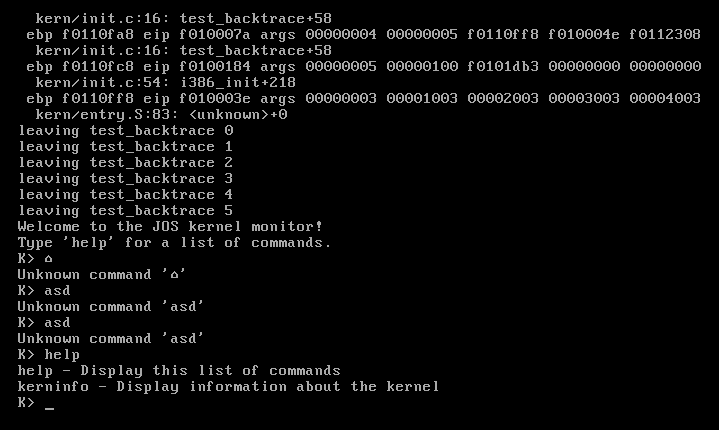
\includegraphics[width=1.0\textwidth]{1.png}
    \caption{نمونه اجرای هسته
    \lr{JOS}
    }
    \label{fig1:output}
\end{figure}
ولی این هسته از روی فایل‌های کامپایل شده از قبل اجرا می شود برای اینکه خودمان هسته را کامپایل کنیم
باید دایرکتوری
\lr{obj}
را پاک کنیم.
و سپس مطمئن شویم که
\lr{gcc}
موجود در سیستم از
\lr{multilib}
پشتیبانی می‌کند.
این کار بسته به
\lr{package manager}
موجود در سیستم به اشکال متفاوتی صورت می‌گیرد.
در توزیع
\lr{Arch}
ما با استفاده از دستور زیر کتابخانه‌های
\lr{multilib}
را نصب کردیم. \pagebreak
\begin{latin}
\begin{lstlisting}[language=bash]
[hossein@TiD lab]$ pacman -S multilib-devel
:: There is 1 member in group multilib-devel:
:: Repository core
   1) lib32-gcc-libs

Enter a selection (default=all):
warning: lib32-gcc-libs-12.2.1-2 is up to date -- reinstalling
resolving dependencies...
looking for conflicting packages...

Packages (1) lib32-gcc-libs-12.2.1-2

Total Download Size:    29.83 MiB
Total Installed Size:  107.61 MiB
Net Upgrade Size:        0.00 MiB
\end{lstlisting}
\end{latin}
همچنین باید پکیج
\lr{qemu}
را نصب کرده تا بتوانیم شبیه‌ساز
\lr{QEMU}
را اجرا کنیم.
در ادامه بعد سعی می‌کنیم تا هسته را با دستور
\lr{make}
کامپایل کنیم که به مشکل زیر برمی‌خوریم.
\begin{figure}[H]
    \centering
    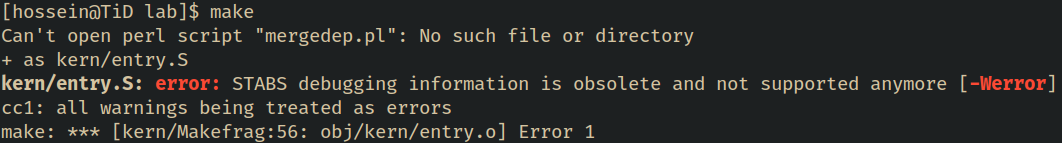
\includegraphics[width=1.0\textwidth]{2.png}
    \caption{نمونه اجرای هسته
    \lr{JOS}
    }
    \label{fig2:output}
\end{figure}
این خطا به ما می‌گوید که اطلاعات دیباگ
\lr{STABS}
در نسخه‌های جدید
\lr{gcc}
ساپورت نمی‌شوند.
در ادامه می‌توانیم از نسخه
\lr{DWARF}
برای این‌کار استفاده کنیم و محدودیتی از این قبال نداریم.
برای اینکار در فایل
\lr{GNUMakefile}
تغییرات زیر را اعمال می‌کنیم.
\begin{latin}
\begin{lstlisting}[language=c]
    <@\textcolor{red}{-CFLAGS += -Wall -Wno-format -Wno-unused -Werror -gstabs -m32}@>
    <@\textcolor{teal}{+CFLAGS += -Wall -Wno-format -Wno-unused -Werror -g -m32}@>
    <@\textcolor{red}{-KERN\_CFLAGS := \$(CFLAGS) -DJOS\_KERNEL -gstabs}@>
    <@\textcolor{red}{-USER\_CFLAGS := \$(CFLAGS) -DJOS\_USER -gstabs}@>
    <@\textcolor{teal}{+KERN\_CFLAGS := \$(CFLAGS) -DJOS\_KERNEL -g}@>
    <@\textcolor{teal}{+USER\_CFLAGS := \$(CFLAGS) -DJOS\_USER -g}@>
\end{lstlisting}
\end{latin}
مشکل بعدی که با آن روبه‌رو می‌شویم در مورد لینکر است.
\begin{latin}
    ld: multiple definition of text\_color; init.o: console.h:20: first defined here
\end{latin}
این ارور بر روی چندین آبجکت نشان داده می‌شود و ارور نیز برای جا شدن در صفحه کوتاه شده است.
برای حل کردن این ارور که مربوط به متغیر گلوبال
\lr{text\_color}
است باید این متغیر را به عنوان
\lr{static}
در فایل
\lr{console.h}
تعریف کنیم.
\begin{figure}[H]
    \centering
    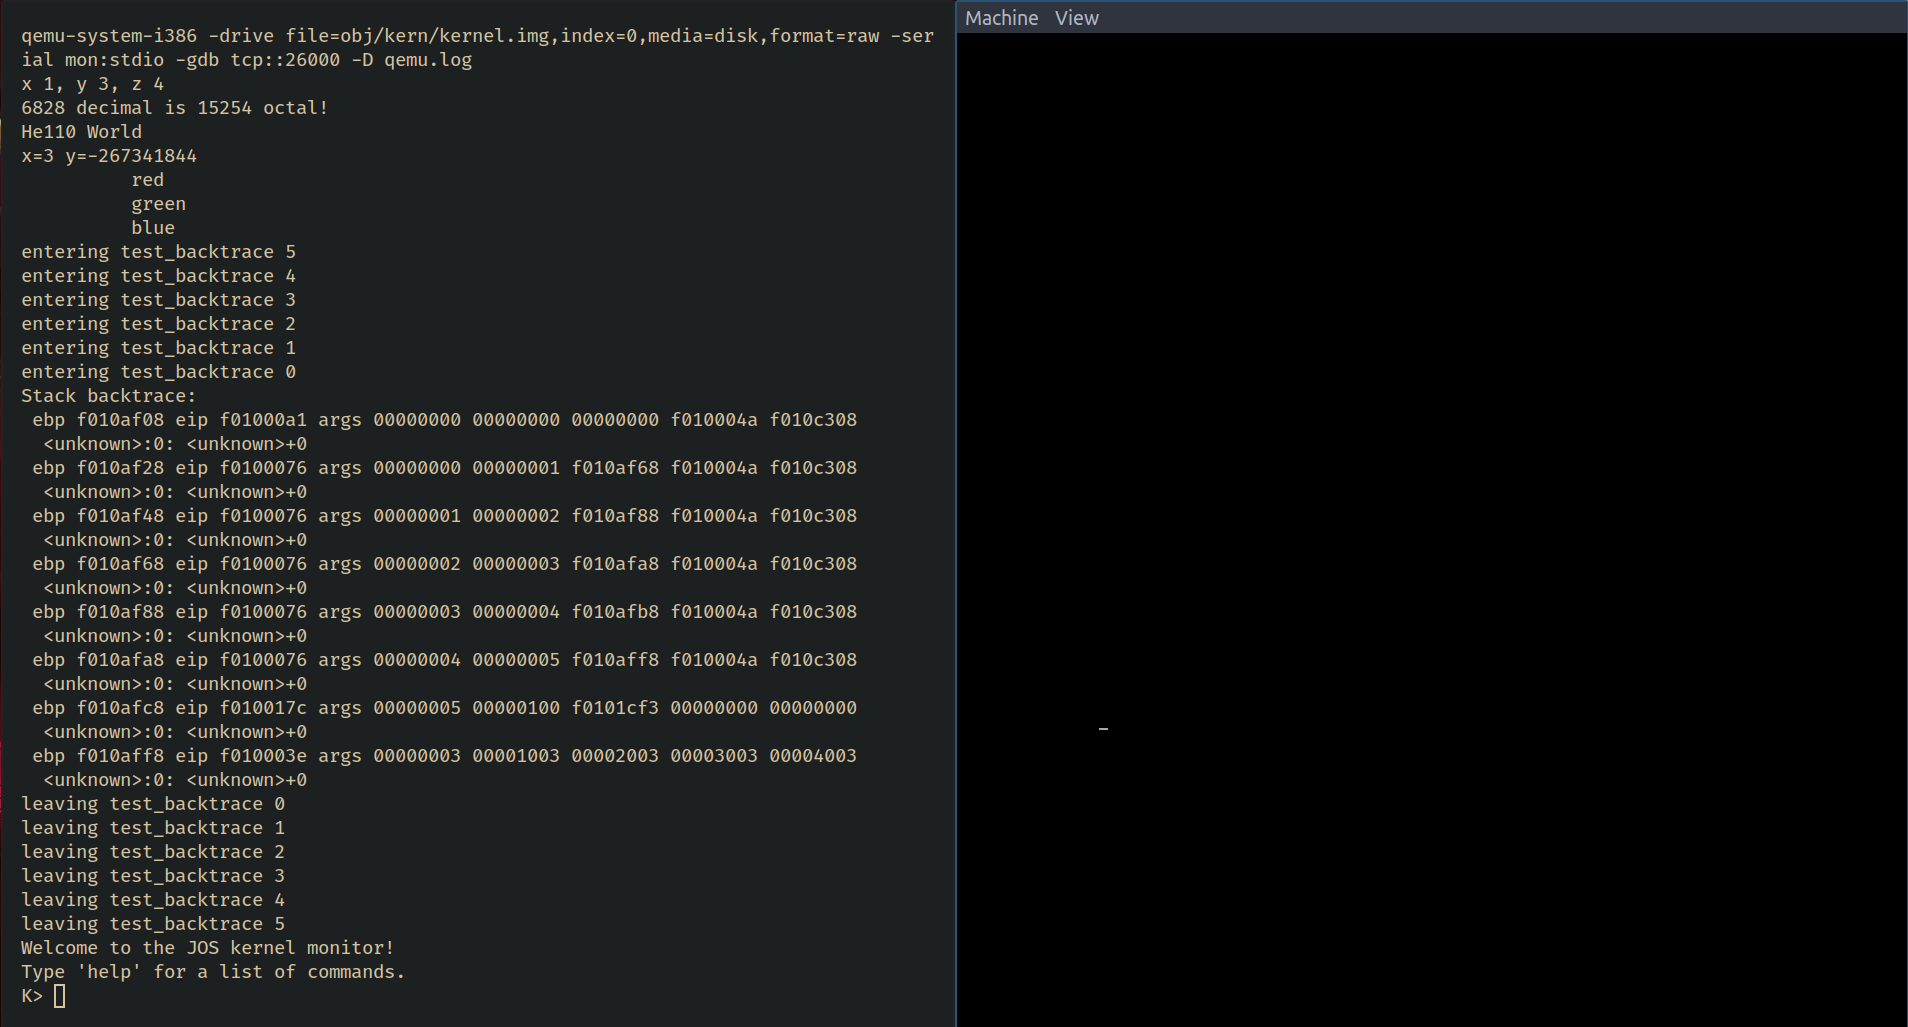
\includegraphics[width=1.0\textwidth]{3.png}
    \caption{نمونه اجرای هسته
    \lr{JOS}
    بعد از حل کردن مشکلات کامپایلری
    }
    \label{fig3:output}
\end{figure}
همانطوری که در صفحه می‌بینید رنگ سفید در
\lr{framebuffer}
اعمال نشده است.
این موضوع به خاطر این است که متغیر مقدار اولیه را به درستی نمی‌گیرد.
برای این کار مقدار اولیه را در هدر به این متغیر می‌دهیم تا در بخش
\lr{.bss}
به درستی ذخیره شود.
مقدار رنگ سفید
\lr{0x700}
است.
\begin{figure}[H]
    \centering
    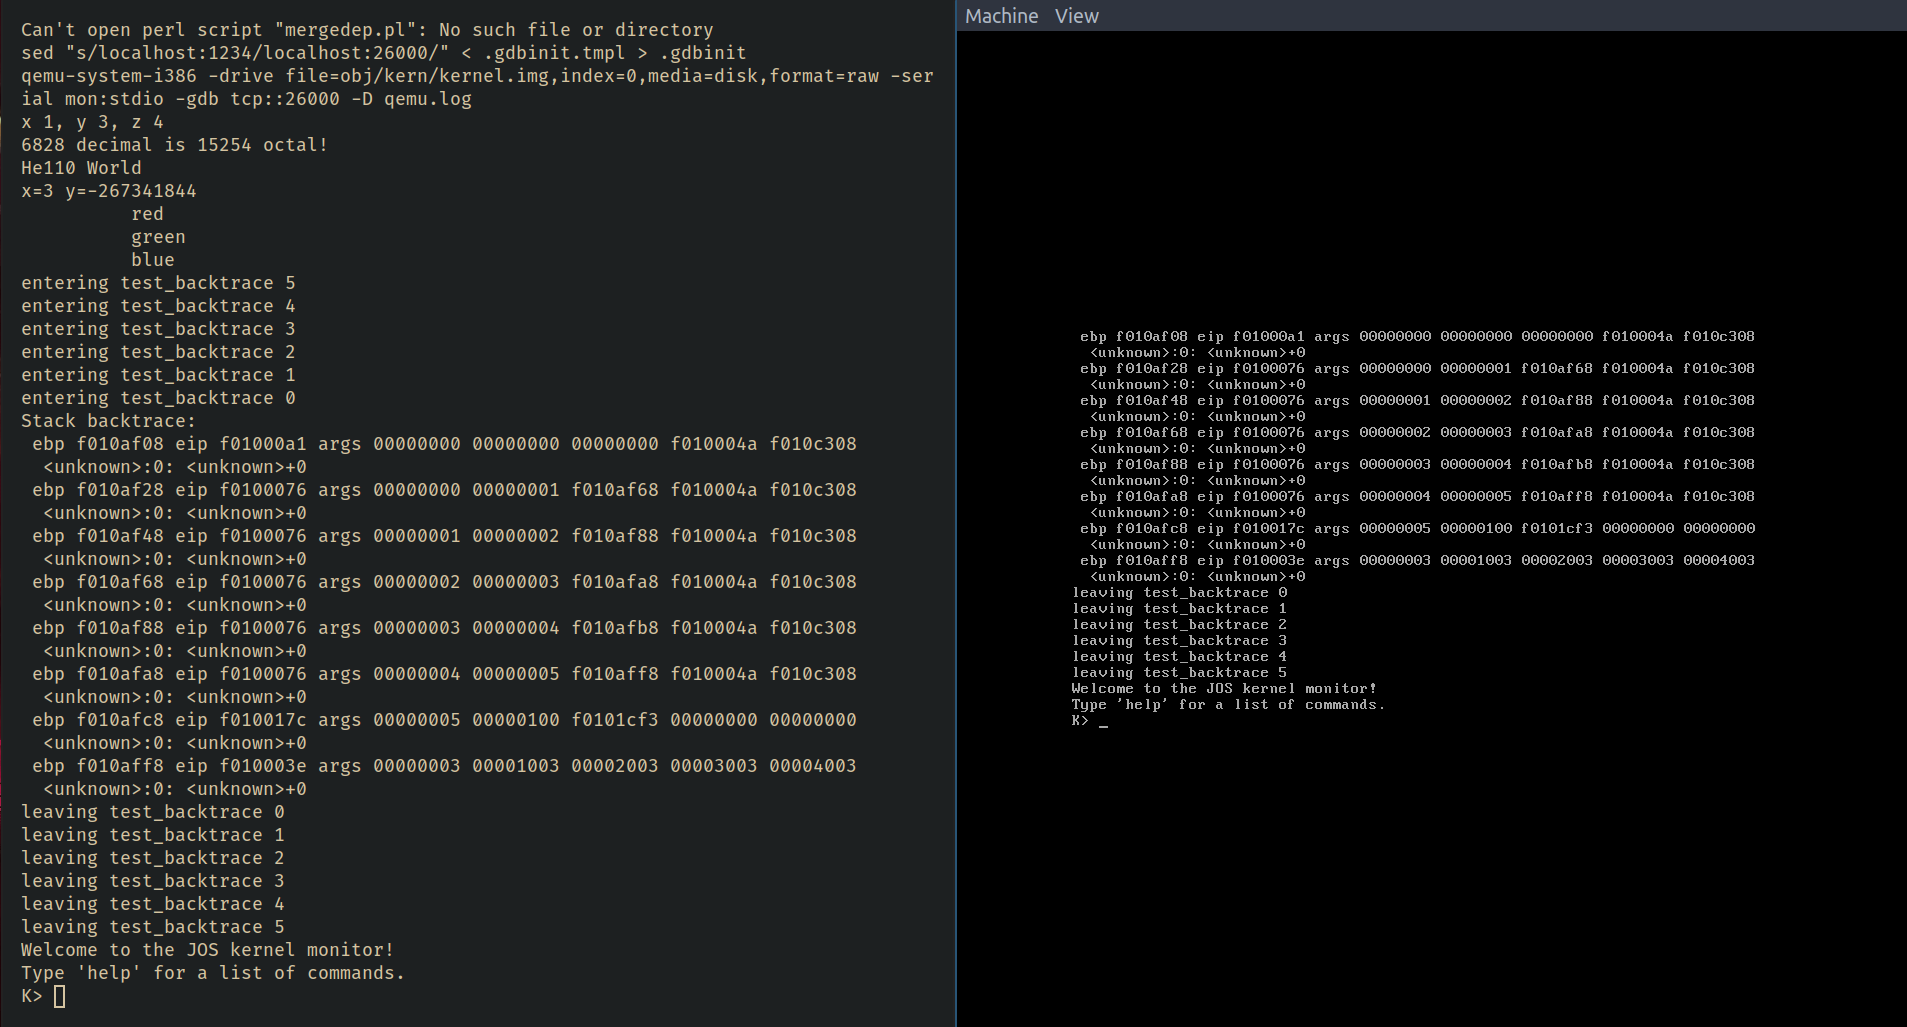
\includegraphics[width=1.0\textwidth]{4.png}
    \caption{نمونه اجرای هسته
    \lr{JOS}
    بعد از حل کردن مشکلات کامپایلری
    و مشکل رنگ
    }
    \label{fig4:output}
\end{figure}
بعد از انجام این مراحل و حل مشکلات کد و مشکلات
\lr{build system}
می‌توانیم در مرحله بعدی به راحتی به این هسته این سیستم عامل کد خودمان را اضافه کنیم.
% \bibliography{references}  % need to put bibtex references in references.bib 
\end{document}
